\documentclass{beamer}
%\usepackage{tikz}
\usepackage{fancyvrb}
\usepackage{mathtools}
\usetheme{CambridgeUS}
\title{QCViewer}
\author{Alex Parent}
\institute{University of Waterloo, IQC}
\date{January 17th, 2012}
\begin{document}

\begin{frame}
\titlepage
\end{frame}

\begin{frame}{Outline}
Quantum Circuit
\begin{itemize}
\item Design
\item Visualization 
\item Simulation  
\end{itemize}
\end{frame}

\begin{frame}{Grover's Algorithm}
\begin{center}
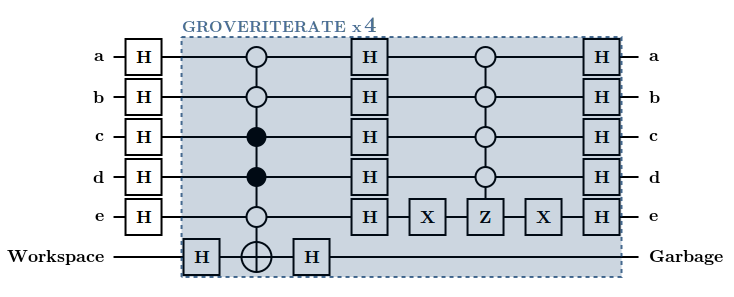
\includegraphics[scale=0.32]{grover_circuit}
\end{center}
\end{frame}

\begin{frame}[fragile]{File Format}

\begin{center}
\begin{tiny}
\begin{BVerbatim}[boxwidth=auto]
.v a b c d e Workspace
.i a b c d e Workspace
.o a b c d e

BEGIN 5H (a, b, c, d, e)
H a; H b; H c; H d; H e
END 5H

BEGIN GroverIterate (a, b, c, d, e, Workspace)
H Workspace
T a' b' c d e' Workspace
H Workspace
5H a b c d e
X e
Z a' b' c' d' e
X e
5H a b c d e
END GroverIterate

BEGIN
H5 a b c d e
GroverIterate^4 a b c d e Workspace
END
\end{BVerbatim}
\end{tiny}

\end{center}

\end{frame}

\begin{frame}{Simulation}
\begin{center}
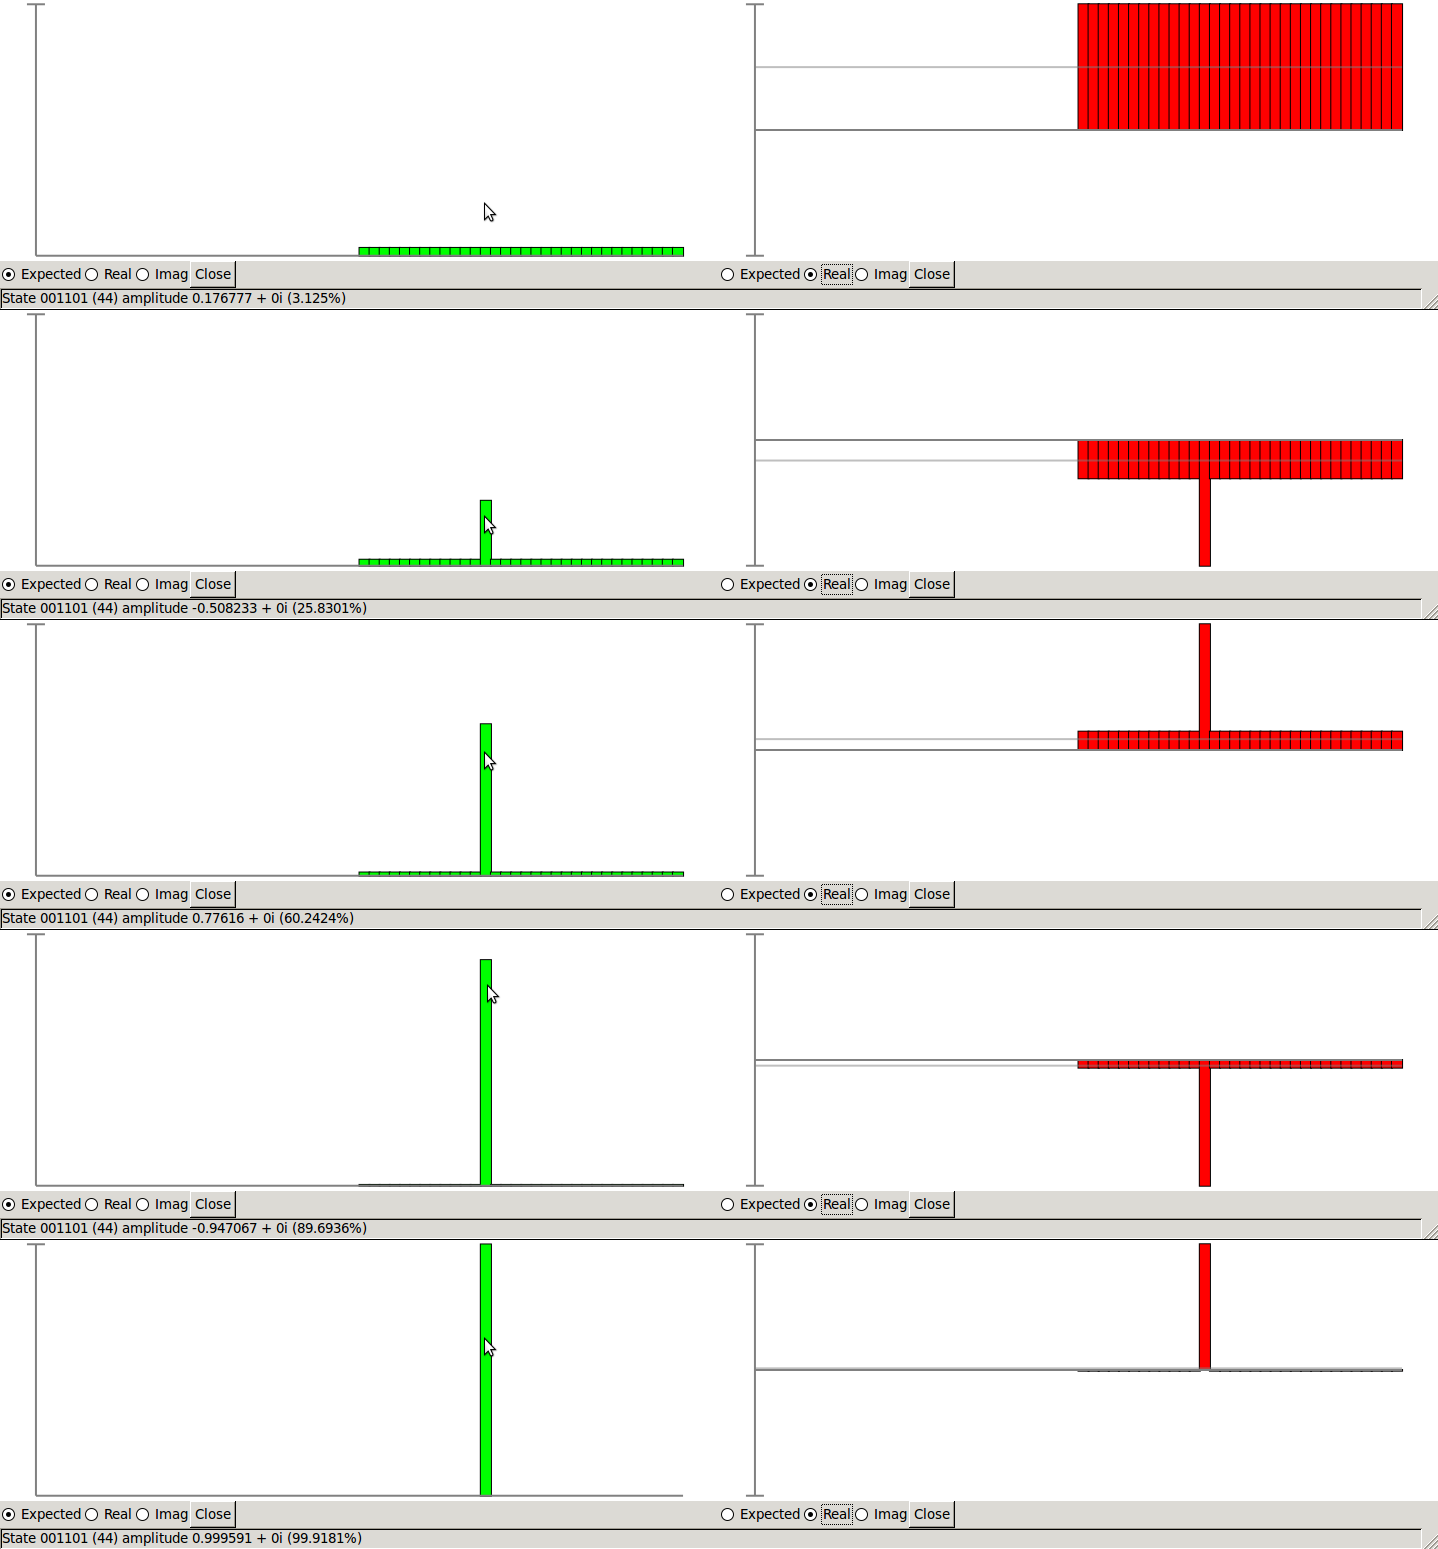
\includegraphics[scale=0.11]{simulate}
\end{center}
\end{frame}


\end{document}
